\chapter{\gls{ner} - Named Entity Recognition}
A named entity is an object that can be referred to and tagged with a predefined entity class label to which the object belongs.
The most common entity classes and tags are \gls{per} for persons, \gls{org} for organizations, \gls{loc}
for geographical locations and \gls{gpe} for geopolitical entities.
The task of Named Entity Recognition (\gls{ner}) is to find \glspl{span} of text that constitute such entity classes or tags \cite{StanfordNLPNER}.

\section{Background}
This section will give an overview over the models that have been used previously and the current state-of-the-art models.
\subsection{Rule-Based Models}\label{subsec:rule-based-models}
Rule-based models were the earliest attempts to recognize named entities in text.
They often used lexical patterns, syntactic features, and domain-specific knowledge such as the following:

\begin{center}
\textit{\textbf{Rule}: If a token is capitalized and the next token is a noun, then the first token is likely a person name.}
\end{center}

While Machine Learning (see \ref{subsec:machine-learning-models}) or Deep Learning approaches (\ref{subsec:deep-learning-models})
dominate the academic debate and research, production use cases today still use hand-crafted rules and query techniques \cite{StanfordNLPNER} to find named entities.
One of the reasons for that is the ambiguity and similarity of entity names and types that confuses even the best \gls{ner} models available.
For instance, \textit{A.G. Edwards} could be both, a \gls{per} or an \gls{org} and the company \textit{Blue Shark} could be falsely identified as an animal.
Another reason is that in some use cases only certain entity types or already known entity names shall be found.
In such cases, it often makes sense to comb through a text with \gls{Regex} patterns or apply other handcrafted query strategies.

\subsection{Machine Learning Models}\label{subsec:machine-learning-models}
There are different types of Machine Learning models for the \gls{ner} task.
\subparagraph{Hidden Markov Models}
Hidden Markov Models or \glspl{HMM} \cite{StanfordNLPNER} are applied to sequences of observations and their respective hidden states.
In the field of \gls{ner}, the observations are the words in a text sequence and their hidden states are
the \gls{ner}-tags such as \gls{per} or \gls{loc} to be predicted.

\begin{figure}[H]   %[h] puts picture right here. 't' stands for to, 'b' stands for bottom
    \centering
    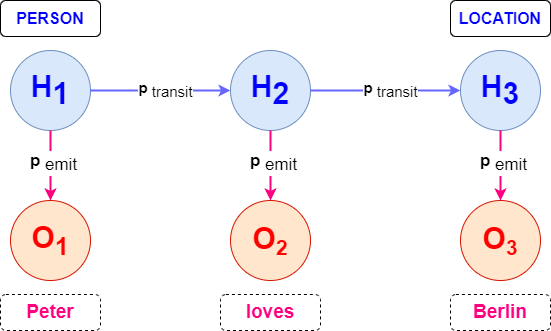
\includegraphics[width=0.5\textwidth]{Assets/HMM}
    \caption{\gls{HMM}: transition/emission probabilities: \textbf{p}\textsubscript{trans}, \textbf{p}\textsubscript{emit}}
    \label{fig:HMM}
\end{figure}

\subparagraph{Conditional Random Fields}
\glspl{CRF} \cite{StanfordNLPNER} belong to the family of \glspl{HMM} and try to address the shortcomings of \glspl{HMM} when it comes to text sequences.
The first problem with a standard \gls{HMM} is that transition and emission probabilities (Fig.\ref{fig:HMM}) are static whereas in text, they are dynamic.
The emission probability that the name of a \gls{per} is \textit{Peter} depends on the context and therefore is dynamic as is the probability that a \gls{loc} comes two words after a \gls{per}.
The second problem is that dependencies are limited in a standard \gls{HMM} meaning that previous hidden states have no direct impact on observations farther away in the sequence.
In a text sequence though, the \gls{ner} tag of the first word in a sentence might have an impact on a word that sits at the end of a sentence.

\begin{figure}[H]   %[h] puts picture right here. 't' stands for to, 'b' stands for bottom
    \centering
    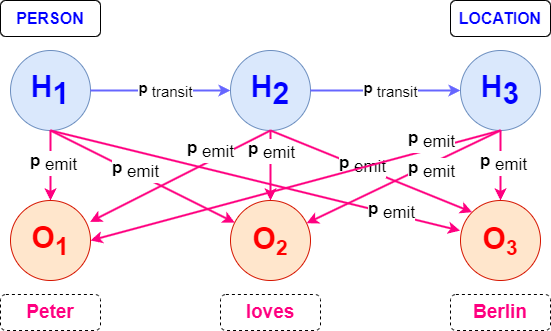
\includegraphics[width=0.55\textwidth]{Assets/CRF}
    \caption{Linear Chain \gls{CRF}}
    \label{fig:CRF}
\end{figure}
A linear chain \gls{CRF} (Fig.\ref{fig:CRF}) overcomes this limitation by allowing emission probabilities from a hidden state (i.e. a \gls{ner} tag) to previous and subsequent observations (i.e. words) but, to avoid computational complexity, prohibits transition probabilities to previous and subsequent hidden states.
The network of emission probabilities and the mapping from the words to the respective \gls{ner} tag is modeled via \textit{\textbf{k}} different feature functions \textbf{f}\textsubscript{j}:

\begin{equation}
f(H_i): \sum\limits_{j=1}^{k} \vec{\textbf{w\textsubscript{j}}} \cdot f_j(O_i, H_{i-1}, H_i, i)  \label{eq:crf1}
\end{equation}

Each feature function has different hidden-state-to-observation \textit{connections} and the model is trained with all vectors \textit{\textbf{w\textsubscript{j}}} as a trainable matrix.
The conditional probability of a certain state \textit{H\textsubscript{i}} (or \gls{ner}-tag) given the observation \textit{O\textsubscript{i}} (or word) and a normalization factor \textit{Z} is calculated by:

\begin{equation}
p(H_i \;| \;O_i) = \frac{1}{Z} \cdot \exp \sum\limits_{l=1}^{n_{words}} \sum\limits_{j=1}^{k} \vec{\textbf{w\textsubscript{j}}} \cdot f_j(O_i, H_{i-1}, H_i, i)  \label{eq:crf2}
\end{equation}

Words as input to a \gls{CRF} model can come in the form of an encoded index from a lookup table or as embedded word vectors \cite{StanfordNLPNER}.

\subsection{Deep Learning Models}\label{subsec:deep-learning-models}

The advent of \glspl{llm} also changed the field of \gls{ner} fundamentally.
Today all leading \gls{ner}-models are based on \gls{Transformer} architectures \cite{leaderboard-ner}.
\glspl{Transformer}, or in more general terms, \gls{ann}-based models can be distinguished between pre-trained models and \glspl{gen-llm}.
Whereas pre-trained models are supervised general purpose \glspl{ann} that are fine-tuned for a specific \gls{ner} task,
\glspl{gen-llm} use the decoder part of a \gls{Transformer} architecture to generate text in response to a \gls{ner}-specific \gls{prompt} request.

\paragraph{Pre-Trained Models}
There are multiple pre-trained models available such as bert-base-NER \cite{bertbaseNER} or NER-BERT \cite{nerbert}, but the one model that stands out in terms of performance and multilingual support is GliNER \cite{gliner}.
GliNER is a light-weight \gls{Transformer} model based on the deBERTa-v3 \cite{deberta} architecture with additional layers for \gls{span} and entity representations.
It was trained with texts from numerous domains and thousands of entity types \cite{gliner} which allows custom entity labels beyond the ones typically found in \gls{ner} models (i.e. \gls{org}, \gls{per}, \gls{loc}, etc.).
GliNER maximizes a combined \gls{token}-\gls{span}-Entity embedding matching score in a computationally efficient way to achieve an O(n log n) complexity.
Because it is available as a spacy wrapper module, it can easily be added to a spacy pipeline.

spacy itself until recently also had a well-performing \gls{ner} component in their pre-trained pipelines (i.e.\emph{en\_core\_web\_sm}, etc.) but performance-wise had to surrender to more recent and specialized models such as GliNER.

GliNER’s multilingual spacy wrapper was used in the project and later compared against a traditional \gls{Regex} model.

\paragraph{\glspl{gen-llm}}\label{par:gpt-ner}
Besides using \glspl{llm} such as the ones from OpenAI directly by sending \gls{prompt} requests, there are also dedicated architectures and indirect ways to extract the named entities from text.

Wang et al \cite{gptner} in 2023 introduced GPT-NER that transforms the \gls{span} labeling task into a text generation task.
For instance, the task of finding \gls{loc} entities in the input text \emph{Columbus is a city}, is transformed to generate the text sequence \emph{@@Columbus\#\# is a city}, where the special \glspl{token} @@ and \#\# surround the entity to be extracted \cite{gptner}.
Before returning the result to the user, the \gls{prompt} also asks the \gls{gen-llm} to self-verify its findings thus decreasing the problem of \glspl{Hallucination}.
The text is then searched for the special \glspl{token} and the model returns the entity in between them.

In the same year, Ashok and Lipton \cite{promptner} introduced PromptNER, which focuses on a specific set of entity types.
The \gls{prompt} provides the model with annotated examples and forces it to justify its findings with the entity type definitions provided.

Most other approaches that I came across, use \glspl{gen-llm} for \gls{ner} in a similar way or concentrate on specific industries or domains.

\section{Code-Implementation}\label{sec:code-implementation}

\subsection{Implementation of Pre-Trained Model}
As GliNER \cite{gliner} is available as a registered spacy plugin (see Section \ref{par:spacy-plugin}), the implementation of it in a spacy pipeline is straightforward.
The name of the plugin is just referenced in the spacy function \emph{enable\_pipe("gliner\_spacy")} within the \emph{api\_gliner()} function (see Python-Code \ref{code:spacy-add-gliner})

\begin{listing}[H]
    \captionof{listing}{api\_gliner()}
    \inputminted[
    firstline=149,
    lastline=158,
    firstnumber=149,
    ]{python}{/media/rainergo/PROJECTS/UASFRA-MS-Thesis/src/B_spacy_pipeline/spacy_pipe_build.py}
    \label{code:spacy-add-gliner}
\end{listing}

and this function is then added to the \emph{build\_pipe()} method (see line 110 of Python-Code \ref{code:spacy-add-gliner-function}) in the \emph{SpacyPipeBuild} class, as outlined in Section \ref{subsec:usage}.

\begin{listing}[H]
    \captionof{listing}{build\_pipe()}
    \inputminted[
    firstline=99,
    lastline=113,
    firstnumber=99,
    ]{python}{/media/rainergo/PROJECTS/UASFRA-MS-Thesis/src/B_spacy_pipeline/spacy_pipe_build.py}
    \label{code:spacy-add-gliner-function}
\end{listing}

\subsection{Implementation of Rule-Base Model}
\paragraph{\gls{Regex}}
As stated previously, in some use cases it might make sense to use rule-based models (see \ref{subsec:rule-based-models}) for \gls{ner}.
Pre-trained \glspl{llm}, that incorporate syntactical and semantic information in their embeddings, are required if entity names are unknown and must be determined in a probabilistic way.
As the company names are provided in advance in this project, rule-based methods such as \glspl{Regex} can be tried for \gls{ner}.

For \gls{Regex} to find desired company names in a text, \gls{Regex} patterns need to be created first.

\gls{Regex} patterns can consist of multiple components and these components can either be mandatory or optional.
One such example is the following:

\begin{center}
\textbf{(Hello)\textbackslash s?(World)*}
\end{center}

The first capturing group contains the word \textit{Hello} and the second the word \textit{World}.
The second group and the space in between the words are optional as these terms are followed by an asterix or a question mark which are \emph{quantifiers}.
The first group is mandatory as an \emph{optional quantifier}, such as ?, *, \{0, n\}, is missing.
In this example, the expression \emph{Hello} or \emph{Hello World} would match the pattern, but the expressions \emph{World} or \emph{Hi World} would not.

Company names can consist of one or multiple words.
To distinguish company names from each other and from non-company names, the company name must be recognizable and distinct.
If a company name consists of more than one word, the central question for \gls{Regex} patterns is which words in the company name must be mandatory and which can be optional.
Let’s consider the following company name example:

\begin{center}
\textbf{Deutsche Telekom AG}
\end{center}

A \gls{Regex} pattern must include at least the first two words combined as the words \emph{Deutsche} and \emph{Telekom} alone are not distinct and are commonly used words.
Let’s consider another example:

\begin{center}
\textbf{Apple Inc.}
\end{center}

Here, the same logic applies: The pattern must include the legal term \emph{Inc.} as otherwise the pattern could find a fruit instead of the company \emph{Apple} whereas in the next example the legal term could be optional:

\begin{center}
\textbf{2CRSI S.A.}
\end{center}

The term \emph{2CRSI} itself is so significant and distinct, that the probability of the same term referring to something else than the given company, is very low.

The optionality of a word in a company name is important for two reasons:
\begin{itemize}
  \item Company names are typically fully mentioned at the beginning of a text but in later sentences might be referred to with just one part of their name.
  \item Company mentions could also be part of a noun term.
\end{itemize}

Let’s consider the following sentences:

\begin{center}
\small{\textit{\underline{ACCENTRO Real Estate AG} today published their better than expected earnings.
\underline{Accentro} had a good first quarter, the \underline{Accentro-stock} climbed 3\% on the stock exchange.}}
\end{center}

A \gls{Regex} pattern that has no optionality for the words \emph{Real Estate AG} would only match the first company mention, but would not match the second and third.
So a good \gls{Regex} pattern might look like this:

\begin{center}
\footnotesize{\textbf{(?:\textbackslash bACCENTRO\textbar Accentro\textbackslash b)\textbackslash s*(?i:\textbackslash bReal\textbackslash b)?\textbackslash s*(?i:\textbackslash bEstate\textbackslash b)?\textbackslash s*(?i:\textbackslash bAG\textbackslash b)?}}
\end{center}

The central word \emph{Accentro} could be upper or title cased, the words \emph{Real}, \emph{Estate}, \emph{AG} are optional and their case could be any.
The \emph{\textbackslash b} means beginning and end of a word and the spaces in between the words are optional.
With such a pattern, all three mentions of the company name in the above example will be matched.

\paragraph{Implementation Details}
As the number of companies to be searched for exceeds 2500, manually creating such regular expression patterns would be very time-consuming.
The function

\begin{center}    
\emph{create\_and\_save\_entity\_patterns()}
\end{center}

in the module \emph{spacy\_input} in the \emph{B\_spacy\_pipeline} folder is particularly dedicated to algorithmically transform company names to \gls{Regex} patterns.


They work as follows:
\begin{enumerate}
  \item The function splits the company name into a list of words.
  \item Each word in this list is classified into one of the following classes:
    \subitem \textbf{Binding}: A conjunction term that links two other words such as \emph{and}, \emph{+}, \emph{-}, \emph{\&} like in \emph{Smith \& Wesson}, \emph{Busch+Lombard AG} or \emph{Basic-Fit N.V.}, etc.
    \subitem \textbf{Person Name Initials} such \emph{A.G.} in \emph{A.G. Edwards}.
    \subitem \textbf{Person Names}: For that, a list of 5000 German and English common first and last names are searched for.
    \subitem \textbf{Legal Terms} such as \emph{AG}, \emph{NV}, \emph{GmbH}, etc for which a legal term list was compiled.
    \subitem \textbf{Industry Hints}: Words that give a hint to the industry the company operates in such as \textbf{buildings}, \textbf{capital}, \textbf{carbon}, \textbf{care}, \textbf{casino}, \textbf{catering}, etc.
    \subitem \textbf{Number Terms} such as 11880 in \emph{11880 Solutions}.
    \subitem \textbf{Significantly Cased Words} such as \emph{SUESS} or \emph{MicroTec}
    \subitem \textbf{Number and Letter Words} such as \emph{4imprint} in \emph{4imprint Group plc.}.
    \subitem \textbf{Articles} such as \emph{The} in \emph{The New York Times}.
    \subitem \textbf{Common Words}: If the word is commonly used according to a list of \emph{5000 most common words} in English and German or if the word is in a list of common company name prefixes and suffixes such as \emph{Global} or \emph{Group}.
    \subitem \textbf{Unknown Words}: Words that do not belong to one of the other classes above.

  \item Once all words of a company name are classified, combination patterns of up to five words are created.
\end{enumerate}

The classification task often is carried out with the help of regular expression patterns itself and Python string functions.\\

As a three-word example, let’s assume the company name is:

\begin{center}
\textbf{4imprint Group plc.}
\end{center}

In the first step, the company name gets split into: [\emph{4imprint}, \emph{Group}, \emph{plc}].
In the second step, each of the three words is classified: \emph{4imprint} is classified as a \emph{Number and Letter word}, \emph{Group} is classified as a \emph{Common Word} and \emph{plc} is classified as \emph{Legal Term}.

\emph{Number and Letter Words} are considered unique and distinct so all other words in that company name can be optional.
The resulting regular expression pattern is:

\begin{center}
\footnotesize{\textbf{(?:\textbackslash b4imprint\textbar4Imprint\textbackslash b)\textbackslash s*(?i:\textbackslash bGroup\textbackslash b)?\textbackslash s*(?i:\textbackslash bplc\textbackslash b)?}}
\end{center}

Let’s consider a four-word example:

\begin{center}
\textbf{Advanced Bitcoin Technologies AG}
\end{center}

In the first step, the company name again gets split into: [\emph{Advanced}, \emph{Bitcoin}, \emph{Technologies}, \emph{AG}]
In the second step, \emph{Advanced} is classified as a \emph{Common Word} as is the word \emph{Technologies}.
\emph{Bitcoin} is classified as an \emph{Industry Hint} and \emph{AG} as a \emph{Legal Term}.
No word from these classes is considered unique and distinct, but the legal classifier is not needed as there is more than one word in the company name.
So the algorithm determines that the first three words are mandatory in the \gls{Regex} pattern and the legal term is optional:

\begin{center}                                                                                                                                                                                                              
\footnotesize{\textbf{(?:\textbackslash bAdvanced\textbackslash b)\textbackslash s*(?:\textbackslash bBitcoin\textbackslash b)\textbackslash s*(?:\textbackslash bTechnologies\textbackslash b)\textbackslash s*(?i:\textbackslash bAG\textbackslash b)?}}
\end{center}


\paragraph{Pattern Naming and Multithreading}
The patterns are saved as \emph{JSONL}-files and are later loaded by a spacy pipeline component that tries to find matches for the patterns in the text.
As the number of companies and thus the number of patterns exceeds 2500, two questions arise:

\begin{enumerate}
    \item How can matches of patterns be mapped to the individual company identifiers and names?
    \item How can over 2500 patterns be efficiently run against each text?
\end{enumerate}

Each \gls{Regex} pattern gets a name that is derived from the company’s unique identifier which is the company stock ticker symbol.


The function \emph{symbol\_to\_groupname\_convert()}
\begin{listing}[H]
    \captionof{listing}{symbol\_to\_groupname\_convert()}
    \inputminted[
    firstline=62,
    lastline=77,
    firstnumber=62,
    ]{python}{/media/rainergo/PROJECTS/UASFRA-MS-Thesis/src/B_spacy_pipeline/spacy_input.py}
    \label{code:symbol-to-groupname-convert}
\end{listing}
first converts the company symbol to a regular expression name which is then prefixed to the pattern that was created above.

For instance: The stock ticker symbol for the company \emph{Advanced Bitcoin Technologies AG} is \emph{ABT.DU}.
The function converts this to a pattern-eligible name which is \emph{SYMB\_ABT\_DOT\_DU} and with it prefixes the regular expression pattern that was created above:

\begin{center}                                                                                                                                                                                                                                                   
\footnotesize{\textbf{(?P\textless SYMB\_ABT\_DOT\_DU\textgreater (?: \break (?:\textbackslash bAdvanced\textbackslash b)\textbackslash s*(?:\textbackslash bBitcoin\textbackslash b)\textbackslash s*(?:\textbackslash bTechnologies\textbackslash b)\textbackslash s*(?i:\textbackslash bAG\textbackslash b)?))}}
\end{center}                                                                                                                                                                                                                                                     

A match against this pattern returns a Python \emph{re match object} that, among other information, contains the pattern’s name.
The pattern’s name then can be re-converted to the company symbol which is attached as extension to the matching \gls{span} or \gls{token} in the Doc-object of the spacy pipeline.

To make this process computationally efficient, the matching algorithm is run concurrently.
The function \emph{run\_re\_finditer\_concurrently()} runs the Python re function \emph{finditer} in parallel and the spacy pipeline component \emph{OwnRegexSearch} applies this concurrent function to each article text:

% Importing code from Python file and overwrite global minted settings

\begin{listing}[H]
    \captionof{listing}{run\_re\_finditer\_concurrently()}
    \inputminted[
    firstline=8,
    lastline=20,
    firstnumber=8,
    ]{python}{/media/rainergo/PROJECTS/UASFRA-MS-Thesis/src/G_utils/concurrency.py}
    \label{code:run-re-finditer-concurrently}
\end{listing}

This match algorithm, that runs over 2500 patterns on each article text, on my standard machine only takes around 500 milliseconds on average per text to execute.

\paragraph{Comparing Rule-Based vs. Pre-Trained vs. \glspl{gen-llm}}
With 500 milliseconds per text, the rule-based method with \gls{Regex} is approximately as fast as the respective GliNER component in spacy’s pre-trained pipeline.
The \gls{Regex} algorithm does not find all companies in the text and is particularly sensitive to misspelled company names, too little optionality in the \gls{Regex} pattern or if company names only consist of one, very common word.


But in most cases, it is as accurate as spacy’s pre-trained GliNER pipeline component and in some cases, particularly if the company name is peculiar and can be confused with subjects from other domains, it is more accurate.
Some shortcomings of the regex approach can be cured if non-working patterns are manually adjusted.
For instance: The company name
\begin{center}
    \textbf{Schott Pharma AG \& Co. KgaA}
\end{center}
contains the person name \emph{Schott} which is uncommon and thus not found in the existing list of person names for the classification task in the \emph{create\_and\_save\_entity\_patterns()} function.
The name \emph{Schott} also starts with a capital letter and is thus considered unique and distinct for which the algorithm allows the other words in the company name to be optional.
The \gls{Regex} pattern could be adjusted by manually adding the name \emph{Schott} to the list of common person names or by requiring the word \emph{Pharma} to be mandatory.

\subsection{Implementation of \gls{gen-llm} model}
For the sake of comparing different approaches, I also tried a \gls{gen-llm} for the \gls{ner} task.
Asked to find named entities in a text, ChatGPT using the OpenAI 4o-mini model with a simple \gls{prompt}, already found most of the entities in a sample text:

\begin{figure}[H]   %[h] puts picture right here. 't' stands for to, 'b' stands for bottom
    \centering                                                                                                                     
    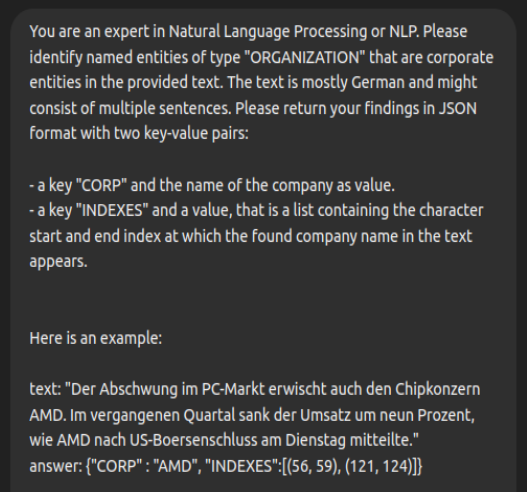
\includegraphics[width=0.9\textwidth]{Assets/chatgpt11}
    \caption{ChatGPT \gls{ner} \gls{prompt} - Part 1}
    \label{fig:chatgpt11}
\end{figure}
\begin{figure}[H]   %[h] puts picture right here. 't' stands for to, 'b' stands for bottom
    \centering
    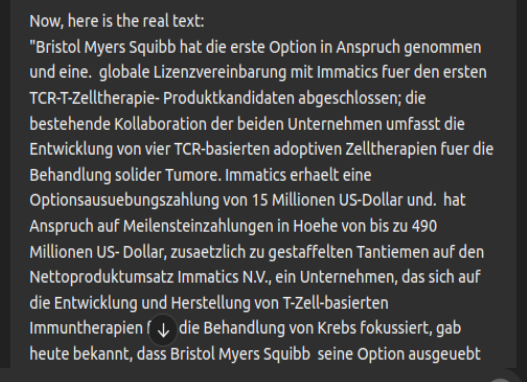
\includegraphics[width=0.9\textwidth]{Assets/chatgpt12}
    \caption{ChatGPT \gls{ner} \gls{prompt} - Part 2}
    \label{fig:chatgpt12}
\end{figure}

\begin{figure}[H]
    \centering                                                  
    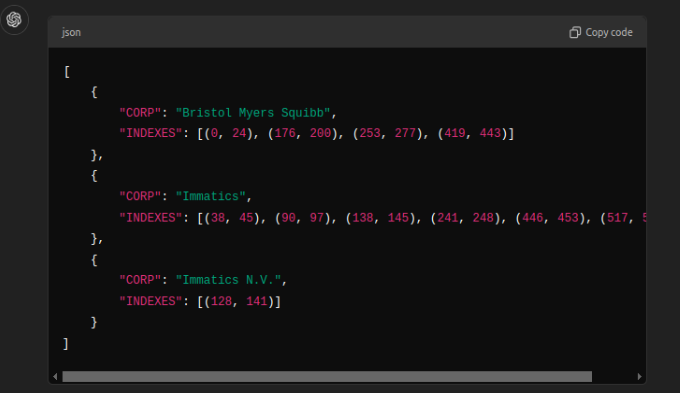
\includegraphics[width=0.9\textwidth]{Assets/chatgpt2}
    \caption{ChatGPT JSON Response}
    \label{fig:chatgpt2}
\end{figure}

But this \gls{gen-llm}-approach for \gls{ner} was inferior to the rule-based \gls{Regex} approach because:

\begin{itemize}
\item It found less entities.
\item It found entities that were not searched for.
\item The latency was higher as the request had to be sent to the OpenAI server first.
\item The position indexes for the found entities were all wrong so locating them would have required an extra step or the usage of OpenAI function tools which would have increased the latency even further.
\item It was more costly as OpenAI charges fees for using their \glspl{llm}.
\item The results were very volatile and unstable as they differed from request to request.
\end{itemize}

Some of these shortcomings can probably be cured by:
\begin{itemize}
\item fine-tuning the \gls{prompt}.
\item providing more few-shot examples.
\item using function tools that are available from most \gls{llm}-providers such as OpenAI.
\item providing a list of entities that shall be searched for.
\item using local, open-source \glspl{llm} and frameworks such as Llama3 \cite{llama3} running on Ollama \cite{ollama} installed on a local machine.
\end{itemize}
Nevertheless, the rule-based approach with \gls{Regex} already delivered very good results and in my assessment is best suited if the company names are given.
This would change if they were not given as then the creation of \gls{Regex} patterns was not possible and a choice would need to be made between a pre-trained and fine-tuned model or a \gls{gen-llm}-approach.

\subsection{Information Extraction Pipeline}
After the \gls{ner} component has run, the spacy pipeline has attached the found company information to the respective custom extensions:
\begin{figure}[H]   %[h] puts picture right here. 't' stands for to, 'b' stands for bottom
    \centering
    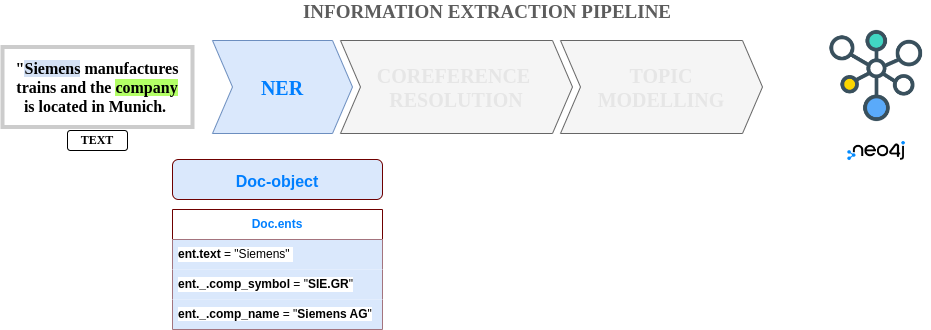
\includegraphics[width=0.85\textwidth]{Assets/pipelineNER}
    \caption{spacy pipeline after \gls{ner} component}
    \label{fig:pipeNER}
\end{figure}
